\scanpage{11}
\mspage{8}
Let us prove (iv). Suppose proved
\[
\pi_{j\alpha}\in\mathcal E\quad\text{for}\quad j\notin[i,2n-i]
\tag{6.7}
\]
where $i\leq n$, and let us prove that
\deleted{\[\pi_{j\alpha}\in\mathcal E\quad\text{for}\quad j\in\]}
\[
\pi_{j\alpha}\in\mathcal E\quad\text{for }j=i\text{ or }j=2n-i,
\tag{6.7'}
\]
which will prove (iv) \inserted{\figure{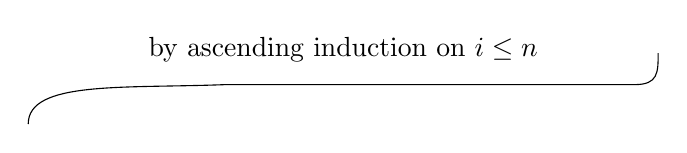
\begin{tikzpicture}[x=1cm,y=1cm]
\node at (0,.25) {by ascending induction on $i\leq n$};
\draw (-4,-.7) .. controls (-4,-.15) and (-2.8,-.25) .. (-1.5,-.2) -- (3.7,-.2) .. controls (4,-.2) and (4,-.05) .. (4,.2);
\end{tikzpicture}}}. To prove $6.8.$ we proceed by descending induction \deleted{\unsure{on}} on $\alpha$, assuming that.
\[
\deleted{\pi_{j\alpha}}\quad\pi_{i,\alpha'}\in\mathcal E,\quad\pi_{2n-i,\alpha'}\in\mathcal E\quad\text{if }\alpha'>\alpha,
\tag{6.8}
\]
and we shall conclude from this that
\[
\pi_{i,\alpha}\in\mathcal E,\quad\pi_{2n-i,\alpha}\in\mathcal E.
\tag{6.8'}
\]
\deleted{For \deleted{must} will indeed prove $(6.7')$, since we can start the induction ($\pi_{i,\alpha}=\pi_{2n-i,\alpha}=0$ if $\alpha$ large). If $\alpha=0$, we win thanks to the relation
\[
\sum_\alpha\pi_{i,\alpha}=\pi_i\quad\text{thus}\quad\pi_{i,0}=\pi_i-\sum_{\alpha\geq1}\pi_{i\alpha},
\tag{6.9}
\]
thus it suffices to consider the case $\alpha\geq1$.}

Set
\[
q_{i,\alpha}=1-\sum_{\alpha'>\alpha}\pi_{i,\alpha'}=\sum_{\alpha'\leq\alpha}\pi_{i,\alpha}
\]
thus thanks to $(6.8)$ we have
\[
q_{i,\alpha}\in\mathcal E\quad\deleted{\unsure{\mathcal E}}
\]
\mspage{10}
